\documentclass[12pt,a4paper]{article}
\usepackage[utf8]{inputenc}
\usepackage[english]{babel}
\usepackage{amsmath}
\usepackage{amsfonts}
\usepackage{amssymb}

\usepackage{graphicx}
\usepackage{caption}
\usepackage{subcaption}

\usepackage{hyperref}
\usepackage{listings}
\usepackage{lmodern}  % for bold teletype font
\usepackage{amsmath}  % for \hookrightarrow
\usepackage{xcolor}   % for \textcolor



\author{Sven Eriksson}
\title{Writeup for Path Planning Project \\ \large{Part of Udacity self driving car nanodegree}}

\setlength{\parindent}{0pt} % Default is 15pt.
\usepackage{parskip}


\begin{document}
\maketitle

This writeup intends to explain what states I am using in my solution, the transition between them and how they generate paths.

\section{States and transitions}

In my path planning solution I am esentially using two state. Lane following and lane change. The lane following state can be split into two parts, an initial state and the main lane following state. The difference is that the inital state does not have transitions to a lane change state.

The lane change states have been implemented as a change lane left and a change lane right state by the use of a parameter describing direction. They are otherwise identical. See figure \ref{fig:stateMachine} for a graphical representation.

\begin{figure}[h!]
  \centering
    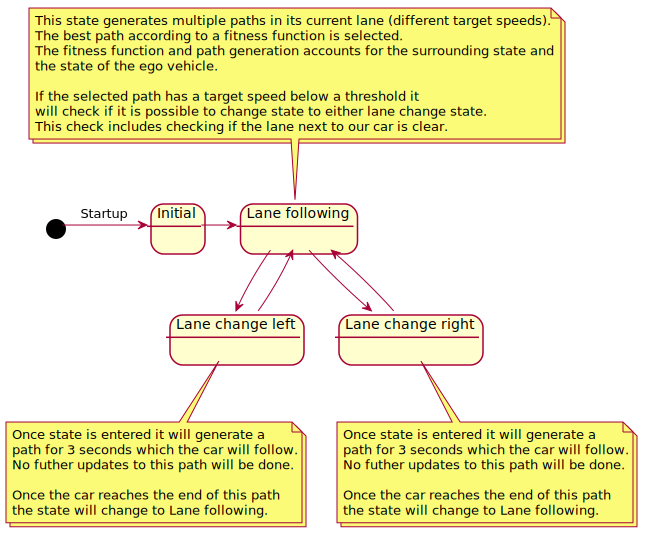
\includegraphics[width=\textwidth]{stateMachine.png}
      \caption{The basic state machine in my solution.}
      \label{fig:stateMachine}
\end{figure}

In the lane following state multiple paths are generated, the main difference between them is the intended final speed. These paths are then evaluated by a fitness function that accounts for speed and acceleration limits as well as the other vehicles. These paths are regenerated and reevaluatet each time the path planner (my code) receives updates from the simulator.

The change lane state generate a single path during upon entry into the state. This is then given to the simulator. It is not replanned based on new information from the simulator.

\subsection{Transition from initial} 
Once the speed of the vehicle reaches a certain threshold (30mph) for the first time the state will transition to lane following.

\subsection{Transition from lane following} 
In the case that the best path has an intended final speed of 43mph or lower and the current speed is 43mph or lower a change lane path will be generated and evaluated by the fitness function. 

If this new change lane path does not violate the limits on velocity and acceleration as well as not collide with any other current vehicle positions a second check will be done. This second check makes sure that the reason for the current lower speed is due to another vehicle in the front of ours and that the lane we a evaluating a transition into is empty for a certain interval around our vehicle in S.

If this second check also succeeds the state will transition to the lane change state. These checks are done for transitions into both lane change left and lane change right independently. Lane change left has priority if both are possible.

\subsection{Transition from lane changing} 
Once the path generated upon entry has too few points left the state will transition back into lane following. The threshold is 25 points (0.5 seconds).

\section{Path generation in states}
The general idea for the two states have been described in the previous section. This section intends to explain the path generation in more detail.

\subsection{Follow lane}
The idea here was to create two splines. One X(t) and one Y(t). First I add a few points to X(t=0.02), ... , X(t=0.2) by using the previously planned points. I add the same interval to Y(t=0.02), ... ,Y(t=0.2). I do an estimation about the S, velocity and D position at t=0.2 based on the previously planned points.

Based on an input parameter finalV I calculate a value of S at two points.

$$S(t=2) = S(t=0.2) + (2-0.2) * (v(t=0.2) + finalV)/2$$
$$S(t=2.5) = S(t=2) + 0.5 * finalV$$

These together with the D for the center of the current lane is then transformed back into X and Y. My two set of points does not contain, X(t=0.02), ... , X(t=0.2), X(t=2) and X(t=2.5). Same time points for Y.

I do now use a spline library to calcute the path for the next 1.5s. I pick points with an interval of 0.02s.

\subsection{Change lane}
The change lane path generation works on more or less the same idea as the follow lane path generation.

The difference is that D at t=2 and t=2.5 is that of the lane that is going to be changed into and that finalV = v(t=0.2).

\newpage
\appendix

\section{Code for path generation}
\lstset{
    frame=tb, % draw a frame at the top and bottom of the code block
    tabsize=4, % tab space width
    showstringspaces=false, % don't mark spaces in strings
    numbers=left, % display line numbers on the left
    commentstyle=\color{green}, % comment color
    keywordstyle=\color{blue}, % keyword color
    stringstyle=\color{red}, % string color
    language=C++,
    breaklines=true,
    postbreak=\mbox{\textcolor{red}{$\hookrightarrow$}\space}
}
\begin{lstlisting}[title=Lane following state path generation]
vector<vector<double>> StayInLane::possiblePath2(vehicleAndMapState &state, double finalV_mph) {
  double extra_t = 0.5;
  double path_t = 2;
  double max_t = 1.5;

  vector<double> X, Y, T;

  vector<double>* previousX = state.previous_path_x;
  vector<double>* previousY = state.previous_path_y;

  int keepNumberOfSteps = 10;

  double t = 0.02;
  double temp_X, temp_Y;
  double initialSpeed;
  double S, D;

  if(previousX->size() > keepNumberOfSteps * 1.5){
    for(int i=0; i<keepNumberOfSteps;i++){
      temp_X = previousX->at(i);
      temp_Y = previousY->at(i);
      X.push_back(temp_X);
      Y.push_back(temp_Y);
      T.push_back(t);
      t += 0.02;
    }
    int deltaSteps = 2;
    dynamics pastPath = dynamicsEstimator(*previousX, *previousY, deltaSteps);

    double S_pos, D_pos;
    vector<double> SD = getFrenet(pastPath.pos.at(keepNumberOfSteps/deltaSteps).X, pastPath.pos.at(keepNumberOfSteps/deltaSteps).Y, deg2rad(state.car_yaw), *state.map_waypoints_x, *state.map_waypoints_y);

    S = SD.at(0);
    initialSpeed = pastPath.vel_abs.at(keepNumberOfSteps/deltaSteps);
  }else{
    X.push_back(state.car_x);
    Y.push_back(state.car_y);
    T.push_back(0);

    S = state.car_s;
    initialSpeed = state.car_speed;
  }

  double finalSpeed = mph2mps(finalV_mph);


  D = middleOfLane(laneNumber(state.car_d));
  S = S + (path_t - t) * (initialSpeed + finalSpeed)/2;

  vector<double> XY = getXY(S, D, *state.map_waypoints_s, *state.map_waypoints_x, *state.map_waypoints_y);
  temp_X = XY.at(0);
  temp_Y = XY.at(1);
  X.push_back(temp_X);
  Y.push_back(temp_Y);
  T.push_back(path_t);

  S = S + extra_t * finalSpeed;

  XY = getXY(S, D, *state.map_waypoints_s, *state.map_waypoints_x, *state.map_waypoints_y);
  temp_X = XY.at(0);
  temp_Y = XY.at(1);
  X.push_back(temp_X);
  Y.push_back(temp_Y);
  T.push_back(path_t + extra_t);


  tk::spline splineX;
  tk::spline splineY;
  splineX.set_points(T, X);
  splineY.set_points(T, Y);

  vector<double> finalX, finalY;

  for(double t=0.02; t<max_t; t+=0.02) {
    finalX.push_back(splineX(t));
    finalY.push_back(splineY(t));
  }

  return {finalX, finalY};
}
\end{lstlisting}

\begin{lstlisting}[title=Lane change state path generation]
vector<vector<double>> ChangeLane::possiblePath(vehicleAndMapState &state, double finalV_mph){

  vector<double>* previousX = state.previous_path_x;
  vector<double>* previousY = state.previous_path_y;

  double t=0.02;
  double max_t = 2;
  double extra_t = 1;
  double delta_t = 1;

  double tempX, tempY;

  double initialS, initialV, initialD, finalS, finalV, finalD, yaw_radian;

  initialS = state.car_s;
  initialV = state.car_speed;
  initialD = state.car_d;

  finalV = mph2mps(finalV_mph);
  initialV = mph2mps(state.car_speed);

  finalD = middleOfLane(laneNumber(state.car_d) + direction);

  if(finalD > 13 || finalD < 1){
    finalD = middleOfLane(laneNumber(state.car_d));
  }

  finalS = initialS + max_t*(initialV + finalV)/2;

  yaw_radian = deg2rad(state.car_yaw);


  vector<double> S, D, T;
  vector<double> X, Y;
  vector<vector<double>> temp;

  X.clear();
  Y.clear();

  double temp_X;
  double temp_Y;
  double speedAfterPrevious;
  double previousS;
  double previousD;

  if(previousX->size()>2){
    for(int i=0; i<previousX->size() && i<25; i++){
      temp_X = previousX->at(i);
      temp_Y = previousY->at(i);
      X.push_back(temp_X);
      Y.push_back(temp_Y);
      T.push_back(t);
      t+=0.02;
    }

    //TODO: This does probably cause some speed fluctiation.
    if(X.size()>11){
      speedAfterPrevious = sqrt(pow(X.at(X.size() - 1) - X.at(X.size() - 11), 2) +
                                pow(Y.at(Y.size() - 1) - Y.at(Y.size() - 11), 2)) / 0.2;
    }else {
      speedAfterPrevious = sqrt(pow(X.at(X.size() - 1) - X.at(X.size() - 2), 2) +
                                pow(Y.at(Y.size() - 1) - Y.at(Y.size() - 2), 2)) / 0.02;
    }
    vector<double> sd = getFrenet(X.back(), Y.back(), state.car_yaw, *state.map_waypoints_x, *state.map_waypoints_y);
    previousS = sd.at(0);
    previousD = sd.at(1);

  }else{
    S.push_back(initialS);
    D.push_back(initialD);
    T.push_back(0);
    previousS = initialS;
    previousD = initialD;

    speedAfterPrevious = mph2mps(state.car_speed);
  }

  S.push_back(previousS + speedAfterPrevious * (max_t-t));
  D.push_back(finalD);
  T.push_back(max_t);

  previousS += speedAfterPrevious * (max_t-t);

  S.push_back(previousS + speedAfterPrevious * extra_t/2);
  D.push_back(finalD);
  T.push_back(max_t + extra_t/2);

  S.push_back(previousS + speedAfterPrevious * extra_t);
  D.push_back(finalD);
  T.push_back(max_t + extra_t);


  temp = getXY(S, D, *state.map_waypoints_s, *state.map_waypoints_x, *state.map_waypoints_y);
  for(int i=0; i<temp.data()[0].size();i++){
    tempX = temp.data()[0].at(i);
    tempY = temp.data()[1].at(i);
    X.push_back(tempX);
    Y.push_back(tempY);
  }

  tk::spline splineX;
  tk::spline splineY;
  splineX.set_points(T, X);
  splineY.set_points(T, Y);

  vector<double> finalX, finalY;

  for(double t_iter=0.02; t_iter<max_t+extra_t; t_iter+=0.02) {
    finalX.push_back(splineX(t_iter));
    finalY.push_back(splineY(t_iter));
  }

  return {finalX, finalY};
}



\end{lstlisting}


\end{document}